\documentclass{article}

\usepackage{graphicx}
\usepackage{tikz}
\usepackage{tikzsymbols}
\usetikzlibrary{calc,patterns,shapes.geometric}
\pagestyle{empty}
\usepackage[margin=0pt]{geometry}
\geometry{papersize={14in,12in}}

\def\centerarc[#1](#2)(#3:#4:#5){\draw[#1] ($(#2)+({#5*cos(#3)},{#5*sin(#3)})$) arc (#3:#4:#5);}

\begin{document}
	\begin{figure}
		\centering
		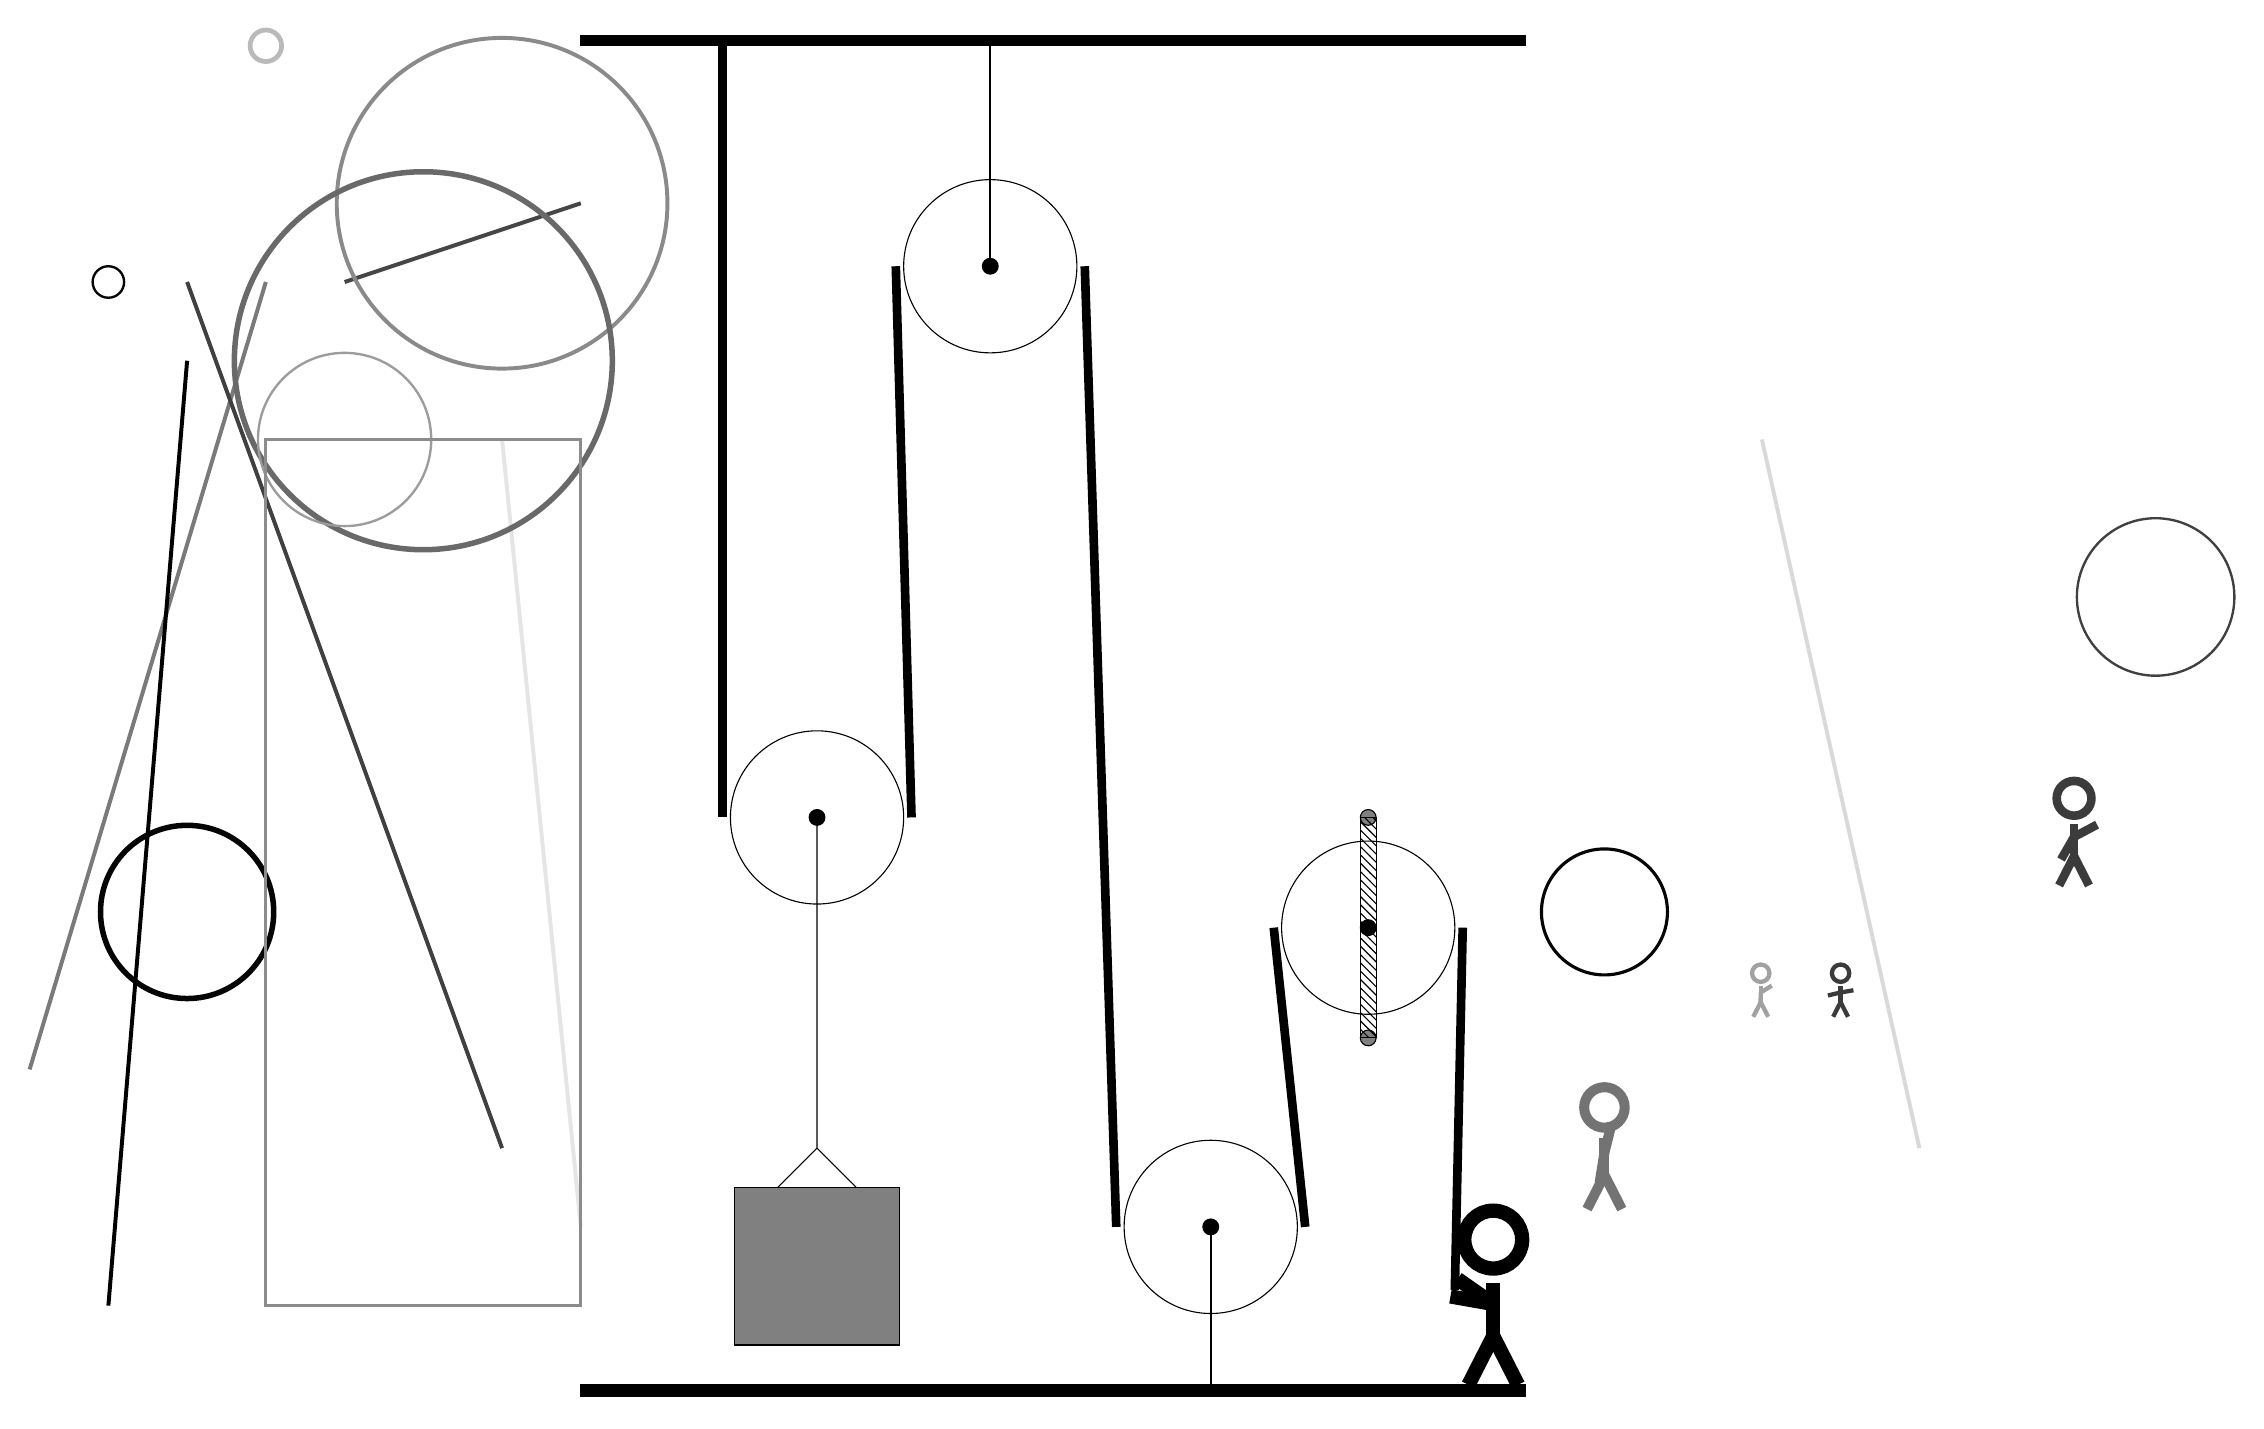
\begin{tikzpicture}
			%%%%% START %%%%%
			
			\draw[fill=black] (-2, 14) rectangle (10, 14.125);
			
			\draw (1, 4.2) circle (1.1);
			\draw[fill=black] (1, 4.2) circle (0.1);
			
			\draw (3.2, 11.2) circle (1.1);
			\draw[fill=black] (3.2, 11.2) circle (0.1);
			\draw[thick] (3.2, 11.2) -- (3.2, 14);
			
			\draw (6, -1) circle (1.1);
			\draw[fill=black] (6, -1) circle (0.1);
			\draw[thick] (6, -1) -- (6, -3);
			
			\draw[fill=white](8, 2.8) circle (1.1);
			\draw[fill=black] (8, 2.8) circle (0.1);
			\draw[fill=black!50] (8, 4.2) circle (0.1);
			\draw[fill=black!50] (8, 1.4) circle (0.1);
			\draw[pattern=north west lines, pattern color=black] (7.9, 4.2) rectangle (8.1, 1.4);
			
			\draw (1, 4.2) -- (1, 0) -- (0.5, -0.5);
			\draw (1, 0) -- (1.5, -0.5);
			\draw[fill=black!50] (-0.05, -0.5) rectangle (2.05, -2.5);
			
			\draw[line width=1.1mm] (-0.2, 14) -- (-0.2, 4.2);
			\centerarc[line width=1.1mm](1, 4.2)(180:360:1.2000000000000002);
			\draw[line width=1.1mm](2.2, 4.2) -- (2.0, 11.2);
			\centerarc[line width=1.1mm](3.2, 11.2)(0:180:1.2000000000000002);
			\draw[line width=1.1mm](4.4, 11.2) -- (4.8, -1);
			\centerarc[line width=1.1mm](6, -1)(180:360:1.2000000000000002);
			\draw[line width=1.1mm](7.2, -1) -- (6.8, 2.8);
			\centerarc[line width=1.1mm](8, 2.8)(0:180:1.2000000000000002);
			\draw[line width=1.1mm](9.2, 2.8) -- (9.1, -1.8);
			
			\draw[line width=0.5mm, color=black!73](-5, 11) -- (-2, 12);
			
			\draw [line width=0.7mm, color=black!98](-7, 3) circle (1.1);
			\draw[line width=0.5mm, color=black!10](-2, -1) -- (-3, 9);
			\draw [line width=0.3mm, color=black!75](18, 7) circle (1.0);
			\node[line width=0.5mm, color=black!77] at (17, 4) {\Strichmaxerl[6][60][28]};
			
			\draw[line width=0.5mm, color=black!52](-6, 11) -- (-9, 1);
			
			\draw[line width=0.5mm, color=black!100](-7, 10) -- (-8, -2);
			
			\draw[line width=0.5mm, color=black!15](15, 0) -- (13, 9);
			\draw [line width=0.3mm, color=black!98](-8, 11) circle (0.2);
			\draw [line width=0.5mm, color=black!46](-3, 12) circle (2.1);
			\draw[line width=0.5mm, color=black!75](-7, 11) -- (-3, 0);
			\draw [line width=0.7mm, color=black!59](-4, 10) circle (2.4);
			\draw [line width=0.6mm, color=black!27](-6, 14) circle (0.2);
			
			\draw [line width=0.3mm, color=black!39](-5, 9) circle (1.1);
			\draw[line width=0.4mm, color=black!45] (-2, 9) rectangle (-6, -2);
			\node[line width=0.3mm, color=black!37] at (13, 2) {\Strichmaxerl[3][89][32]};
			\draw [line width=0.4mm, color=black!98](11, 3) circle (0.8);
			\node[line width=0.6mm, color=black!55] at (11, 0) {\Strichmaxerl[7][81][76]};
			\node[line width=0.7mm, color=black!77] at (14, 2) {\Strichmaxerl[3][13][10]};
			
			
			\node at (9.5, -1.9) {\Strichmaxerl[10][-35][170]};
			
			\draw[fill=black] (-2, -3) rectangle (10, -3.15);
			
			%%%%% END %%%%%
		\end{tikzpicture}
	\end{figure}	
\end{document}